%%%%%%%% ICML 2025 EXAMPLE LATEX SUBMISSION FILE %%%%%%%%%%%%%%%%%

\documentclass{article}

% Recommended, but optional, packages for figures and better typesetting:
\usepackage{microtype}
\usepackage{graphicx}
\usepackage{subfigure}
\usepackage{booktabs} % for professional tables

% hyperref makes hyperlinks in the resulting PDF.
% If your build breaks (sometimes temporarily if a hyperlink spans a page)
% please comment out the following usepackage line and replace
% \usepackage{icml2025} with \usepackage[nohyperref]{icml2025} above.
\usepackage{hyperref}


% Attempt to make hyperref and algorithmic work together better:
\newcommand{\theHalgorithm}{\arabic{algorithm}}

% Use the following line for the initial blind version submitted for review:
% \usepackage{icml2025}

% If accepted, instead use the following line for the camera-ready submission:
\usepackage[accepted]{icml2025}

% For theorems and such
\usepackage{amsmath}
\usepackage{amssymb}
\usepackage{mathtools}
\usepackage{amsthm}

% if you use cleveref..
\usepackage[capitalize,noabbrev]{cleveref}

%%%%%%%%%%%%%%%%%%%%%%%%%%%%%%%%
% THEOREMS
%%%%%%%%%%%%%%%%%%%%%%%%%%%%%%%%
\theoremstyle{plain}
\newtheorem{theorem}{Theorem}[section]
\newtheorem{proposition}[theorem]{Proposition}
\newtheorem{lemma}[theorem]{Lemma}
\newtheorem{corollary}[theorem]{Corollary}
\theoremstyle{definition}
\newtheorem{definition}[theorem]{Definition}
\newtheorem{assumption}[theorem]{Assumption}
\theoremstyle{remark}
\newtheorem{remark}[theorem]{Remark}

% Todonotes is useful during development; simply uncomment the next line
%    and comment out the line below the next line to turn off comments
%\usepackage[disable,textsize=tiny]{todonotes}
\usepackage[textsize=tiny]{todonotes}


% The \icmltitle you define below is probably too long as a header.
% Therefore, a short form for the running title is supplied here:
\icmltitlerunning{OTCE: Hybrid SSM and Attention with Cross Domain Mixture of Experts to construct Observer-Thinker-Conceiver-Expresser for ICML 2025}

\begin{document}

\twocolumn[
\icmltitle{Re-Examine Hybrid State-Space and Self-Attention for In-Context Learning}

% It is OKAY to include author information, even for blind
% submissions: the style file will automatically remove it for you
% unless you've provided the [accepted] option to the icml2025
% package.

% List of affiliations: The first argument should be a (short)
% identifier you will use later to specify author affiliations
% Academic affiliations should list Department, University, City, Region, Country
% Industry affiliations should list Company, City, Region, Country

% You can specify symbols, otherwise they are numbered in order.
% Ideally, you should not use this facility. Affiliations will be numbered
% in order of appearance and this is the preferred way.
\icmlsetsymbol{equal}{*}

\begin{icmlauthorlist}
\icmlauthor{Jingze Shi}{equal,yyy}
\icmlauthor{Bingheng Wu}{equal,yyy,comp}

%\icmlauthor{}{sch}
%\icmlauthor{}{sch}
\end{icmlauthorlist}

\icmlaffiliation{yyy}{Department of XXX, University of YYY, Location, Country}
\icmlaffiliation{comp}{Company Name, Location, Country}
\icmlaffiliation{sch}{School of ZZZ, Institute of WWW, Location, Country}

\icmlcorrespondingauthor{Firstname1 Lastname1}{first1.last1@xxx.edu}
\icmlcorrespondingauthor{Firstname2 Lastname2}{first2.last2@www.uk}

% You may provide any keywords that you
% find helpful for describing your paper; these are used to populate
% the "keywords" metadata in the PDF but will not be shown in the document
\icmlkeywords{Machine Learning, ICML}

\vskip 0.3in
]



\begin{abstract}
% 最近的研究表明, 将状态空间算法驱动的 Mamba 与自注意力算法驱动的 Transformer 相结合, 在大多数语言建模任务上的表现超越了单独使用 Mamba 或 Transformer. 
% 但是, 目前主流的混合建模架构模型在情景学习任务上的表现并不理想, 我们重新审视了这两种算法的优势和劣势, 从原理出发对这种混合建模的结构重新设计. 
% 最终, 重新设计的架构, 在标准短文本任务中提升了 1.3 \% 效果, 在自然长文本任务中提升了 20.86 \% 效果, 在合成长文本任务中提升了 27.06 \% 效果.
Recent research has shown that combining the state-space algorithm-driven Mamba with the self-attention algorithm-driven Transformer outperforms using Mamba or Transformer alone in most language modeling tasks. However, the performance of the mainstream hybrid modeling architecture models in in-context learning tasks is not ideal. We re-examine the advantages and disadvantages of these two algorithms and redesign the structure of this hybrid modeling from the principle. The finally redesigned architecture improves the performance by 1.3\% in standard short text tasks, 20.86\% in natural long text tasks, and 27.06\% in synthetic long text tasks.
\end{abstract}

\section{Introduction}
\label{submission}

The Transformers (Attention is All You Need~\cite{transformer2017}) architecture is popular in modern deep learning language modeling, which can directly capture the relationship between any two elements in a sequence, effectively handle long-distance dependencies, however, the architecture has two main drawbacks. First, when processing long sequences, its self-attention mechanism's quadratic complexity and cache size limit the ability to handle long contexts. Second, Transformer lacks a single summary state, which means that each generated token must compute over the entire context, which exacerbates the model's computational burden.
Meanwhile, the Selective State Model (Mamba~\cite{gu2023mamba}) has emerged. Mamba achieves linear scaling of sequence length during training and maintains a constant state size during generation through its selective state update mechanism. Moreover, due to its linear recursive state update mechanism, Mamba has a single summary state. However, Mamba also has a major drawback, that is, its positional information depends on the implicit local positional information provided by the causal convolution, while long-distance dependencies depend on the matrix D that skips the connection between input and output. This makes Mamba perform poorly in capturing long-distance dependencies, such as correctly capturing input-output formats in context learning (ICL).
An efficient model must have a small state, and an effective model must have a state that contains all the necessary information from the context. To build a model that is both efficient and effective, the key is to design a state that is both compact and comprehensive in capturing the necessary context information. Our main goal is to combine self-attention and the Selective State Model to overcome their respective limitations, further combine them with a mixed expert with extensive general and cross-domain knowledge to build a better basic model architecture than Transformers or Mamba. The model has the ability to learn long context dependencies, aggregate states, and efficient reasoning. This paper proposes a bionic perspective, aiming to explore new model architectures by cleverly combining the Selective State Model with self-attention mechanism. This approach can fully utilize the advantages of the two mechanisms and promote language modeling in a more efficient and effective direction.

\subsection{Positional Information}

We first identified a key challenge in combining the Selective State Model with self-attention: the effective integration of positional information. In Mamba, positional information is provided by the implicit local positional information from the causal convolution, while self-attention itself cannot provide positional information, it relies on positional encoding to provide global positional context. To address this issue, we designed a relative positional information injection method that connects the inner product state of the Selective State Space with the inner product state of self-attention, allowing the input gate-state-output gate of the Selective State Space to make filtered relevant information have discrete relative positional information, and in self-attention, the discrete relative positional information is re-continuous to build long-term dependency relationships of relevant information. This method not only enables our model to have the ability to selectively process input sequences but also effectively capture long-distance dependency relationships. In complex multi-query associative recall tasks, our model trained on the same dataset outperforms larger-scale Mamba, Transformer models, and models that mix Mamba and Transformer without our proposed relative positional information injection method.

\subsection{Cross-Domain Mixture of Experts}
In human society, knowledge is widely distributed across different domains, and these domains are interconnected through common foundational knowledge and cross-domain connections. To simulate this phenomenon in the model, we designed two types of cross-domain mixed experts: Cohesive Cross-Domain Expert and Expansive Cross-Domain Expert. These experts (multi-layer perceptrons) store and transfer common foundational knowledge and cross-domain knowledge between different domains by sharing parameters. The Cohesive Cross-Domain Expert achieves close integration between domains by sharing linear layer parameters within all experts, which is more suitable for small-scale models with fewer experts because of its faster computation speed. The Expansive Cross-Domain Expert shares a complete MLP parameter, adding a common domain knowledge gate in each expert to control the flow of common domain knowledge into private MLP parameters, which is more suitable for large-scale models with more experts because it allows for more flexible adjustment and utilization of common knowledge. Experimental results show that the performance of these two cross-domain mixed experts on the same dataset is better than shared expert isolated mixed experts, confirming the effectiveness of our design in promoting cross-domain knowledge transfer and improving model generalization.

\subsection{Architecture Design}

From a biological perspective, the relationship between input and output can be described by observing, thinking, conceiving, and expressing four stages. Inspired by this idea, we designed a new architecture with a bionic perspective: Observer-Thinker-Conceiver-Expresser (\textbf{OTCE}). The OTCE architecture mimics the natural process of information processing in biology, aiming to optimize information processing and transmission in a modular way. In the Observer module, we use the selective state space's selection ability to filter out irrelevant information in the sequence to retain relevant information. In the Thinker module, we use the self-attention's ability to capture dependencies between any two elements in a sequence of any length, regardless of their position in the sequence, to build long-term dependency relationships. In the Conceiver module, we use the linear recursive state update mechanism of the state space to build a single summary state information. In the Expresser module, we combine the context-aware state information produced by self-attention considering all elements with the summary state information to build a context-aware summary state. We also studied the combination of the Selective State Space and self-attention with ordinary multi-layer perceptrons and cross-domain mixed experts, and finally determined a model combination with the lowest perplexity at the same parameter scale.

We empirically validated OTCE on multiple tasks, including semantic similarity evaluation, long-short text classification, natural language inference, keyword recognition, different domain selection tasks, context learning, and multi-query associative recall tasks. These experiments demonstrate the effectiveness of the OTCE architecture in handling complex language tasks.




\begin{figure}[H]
   \centering
   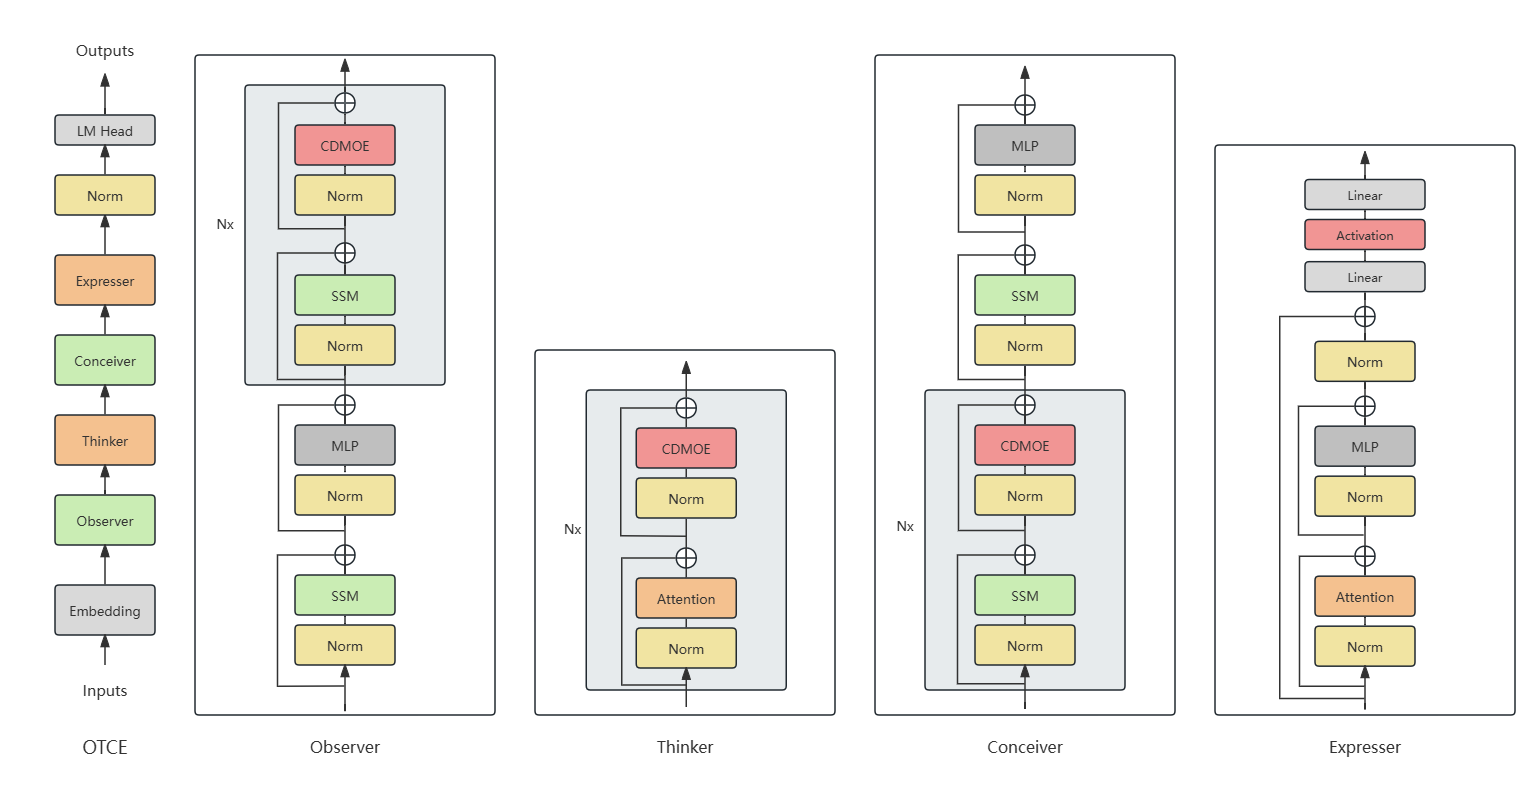
\includegraphics[width=1.0\linewidth]{fig/otce.png}
   \caption{(\textbf{OTCE Architecture}.) OTCE demonstrates the overall combined architecture and process of using Observer, Thinker, Conceiver, and Expresser modules in language modeling tasks. Observer, Thinker, Conceiver, and Expresser show their internal combination of selective state space, self-attention, multi-layer perceptron, and cross-domain mixed experts.}
   \label{fig:otce}
\end{figure}



\section{Background}
\subsection{Selective State Space Models}


Selective state space models~\cite{gu2023mamba} consider that a fundamental problem in sequence modeling is to compress the context into a smaller state. From this perspective, the attention mechanism of Transformers explicitly stores the entire context information, as if reviewing all previous inputs and generated tokens before writing each token. In contrast, RNNs only refer to a fixed number of previous tokens each time, which allows for faster writing but may forget key tokens.

In the precursor state space models of selective state space models, there are 4 parameters$(\Delta t, A, B, C)$, and they do not change with the input. These parameters control the following two stages:





% Note use of \abovespace and \belowspace to get reasonable spacing
% above and below tabular lines.

\begin{table}[t]
\caption{Classification accuracies for naive Bayes and flexible
Bayes on various data sets.}
\label{sample-table}
\vskip 0.15in
\begin{center}
\begin{small}
\begin{sc}
\begin{tabular}{lcccr}
\toprule
Data set & Naive & Flexible & Better? \\
\midrule
Breast    & 95.9$\pm$ 0.2& 96.7$\pm$ 0.2& $\surd$ \\
Cleveland & 83.3$\pm$ 0.6& 80.0$\pm$ 0.6& $\times$\\
Glass2    & 61.9$\pm$ 1.4& 83.8$\pm$ 0.7& $\surd$ \\
Credit    & 74.8$\pm$ 0.5& 78.3$\pm$ 0.6&         \\
Horse     & 73.3$\pm$ 0.9& 69.7$\pm$ 1.0& $\times$\\
Meta      & 67.1$\pm$ 0.6& 76.5$\pm$ 0.5& $\surd$ \\
Pima      & 75.1$\pm$ 0.6& 73.9$\pm$ 0.5&         \\
Vehicle   & 44.9$\pm$ 0.6& 61.5$\pm$ 0.4& $\surd$ \\
\bottomrule
\end{tabular}
\end{sc}
\end{small}
\end{center}
\vskip -0.1in
\end{table}

Tables contain textual material, whereas figures contain graphical material.
Specify the contents of each row and column in the table's topmost
row. Again, you may float tables to a column's top or bottom, and set
wide tables across both columns. Place two-column tables at the
top or bottom of the page.

\subsection{Theorems and such}
The preferred way is to number definitions, propositions, lemmas, etc. consecutively, within sections, as shown below.
\begin{definition}
\label{def:inj}
A function $f:X \to Y$ is injective if for any $x,y\in X$ different, $f(x)\ne f(y)$.
\end{definition}
Using \cref{def:inj} we immediate get the following result:
\begin{proposition}
If $f$ is injective mapping a set $X$ to another set $Y$, 
the cardinality of $Y$ is at least as large as that of $X$
\end{proposition}
\begin{proof} 
Left as an exercise to the reader. 
\end{proof}
\cref{lem:usefullemma} stated next will prove to be useful.
\begin{lemma}
\label{lem:usefullemma}
For any $f:X \to Y$ and $g:Y\to Z$ injective functions, $f \circ g$ is injective.
\end{lemma}
\begin{theorem}
\label{thm:bigtheorem}
If $f:X\to Y$ is bijective, the cardinality of $X$ and $Y$ are the same.
\end{theorem}
An easy corollary of \cref{thm:bigtheorem} is the following:
\begin{corollary}
If $f:X\to Y$ is bijective, 
the cardinality of $X$ is at least as large as that of $Y$.
\end{corollary}
\begin{assumption}
The set $X$ is finite.
\label{ass:xfinite}
\end{assumption}
\begin{remark}
According to some, it is only the finite case (cf. \cref{ass:xfinite}) that is interesting.
\end{remark}
%restatable

\subsection{Citations and References}

Please use APA reference format regardless of your formatter
or word processor. If you rely on the \LaTeX\/ bibliographic
facility, use \texttt{natbib.sty} and \texttt{icml2025.bst}
included in the style-file package to obtain this format.

Citations within the text should include the authors' last names and
year. If the authors' names are included in the sentence, place only
the year in parentheses, for example when referencing Arthur Samuel's
pioneering work \yrcite{Samuel59}. Otherwise place the entire
reference in parentheses with the authors and year separated by a
comma \cite{Samuel59}. List multiple references separated by
semicolons \cite{kearns89,Samuel59,mitchell80}. Use the `et~al.'
construct only for citations with three or more authors or after
listing all authors to a publication in an earlier reference \cite{MachineLearningI}.

Authors should cite their own work in the third person
in the initial version of their paper submitted for blind review.
Please refer to \cref{author info} for detailed instructions on how to
cite your own papers.

Use an unnumbered first-level section heading for the references, and use a
hanging indent style, with the first line of the reference flush against the
left margin and subsequent lines indented by 10 points. The references at the
end of this document give examples for journal articles \cite{Samuel59},
conference publications \cite{langley00}, book chapters \cite{Newell81}, books
\cite{DudaHart2nd}, edited volumes \cite{MachineLearningI}, technical reports
\cite{mitchell80}, and dissertations \cite{kearns89}.

Alphabetize references by the surnames of the first authors, with
single author entries preceding multiple author entries. Order
references for the same authors by year of publication, with the
earliest first. Make sure that each reference includes all relevant
information (e.g., page numbers).

Please put some effort into making references complete, presentable, and
consistent, e.g. use the actual current name of authors.
If using bibtex, please protect capital letters of names and
abbreviations in titles, for example, use \{B\}ayesian or \{L\}ipschitz
in your .bib file.

\section*{Accessibility}
Authors are kindly asked to make their submissions as accessible as possible for everyone including people with disabilities and sensory or neurological differences.
Tips of how to achieve this and what to pay attention to will be provided on the conference website \url{http://icml.cc/}.

\section*{Software and Data}

If a paper is accepted, we strongly encourage the publication of software and data with the
camera-ready version of the paper whenever appropriate. This can be
done by including a URL in the camera-ready copy. However, \textbf{do not}
include URLs that reveal your institution or identity in your
submission for review. Instead, provide an anonymous URL or upload
the material as ``Supplementary Material'' into the OpenReview reviewing
system. Note that reviewers are not required to look at this material
when writing their review.

% Acknowledgements should only appear in the accepted version.
\section*{Acknowledgements}

\textbf{Do not} include acknowledgements in the initial version of
the paper submitted for blind review.

If a paper is accepted, the final camera-ready version can (and
usually should) include acknowledgements.  Such acknowledgements
should be placed at the end of the section, in an unnumbered section
that does not count towards the paper page limit. Typically, this will 
include thanks to reviewers who gave useful comments, to colleagues 
who contributed to the ideas, and to funding agencies and corporate 
sponsors that provided financial support.

\section*{Impact Statement}

Authors are \textbf{required} to include a statement of the potential 
broader impact of their work, including its ethical aspects and future 
societal consequences. This statement should be in an unnumbered 
section at the end of the paper (co-located with Acknowledgements -- 
the two may appear in either order, but both must be before References), 
and does not count toward the paper page limit. In many cases, where 
the ethical impacts and expected societal implications are those that 
are well established when advancing the field of Machine Learning, 
substantial discussion is not required, and a simple statement such 
as the following will suffice:

``This paper presents work whose goal is to advance the field of 
Machine Learning. There are many potential societal consequences 
of our work, none which we feel must be specifically highlighted here.''

The above statement can be used verbatim in such cases, but we 
encourage authors to think about whether there is content which does 
warrant further discussion, as this statement will be apparent if the 
paper is later flagged for ethics review.


% In the unusual situation where you want a paper to appear in the
% references without citing it in the main text, use \nocite
\nocite{langley00}

\bibliography{paper}
\bibliographystyle{icml2025}


%%%%%%%%%%%%%%%%%%%%%%%%%%%%%%%%%%%%%%%%%%%%%%%%%%%%%%%%%%%%%%%%%%%%%%%%%%%%%%%
%%%%%%%%%%%%%%%%%%%%%%%%%%%%%%%%%%%%%%%%%%%%%%%%%%%%%%%%%%%%%%%%%%%%%%%%%%%%%%%
% APPENDIX
%%%%%%%%%%%%%%%%%%%%%%%%%%%%%%%%%%%%%%%%%%%%%%%%%%%%%%%%%%%%%%%%%%%%%%%%%%%%%%%
%%%%%%%%%%%%%%%%%%%%%%%%%%%%%%%%%%%%%%%%%%%%%%%%%%%%%%%%%%%%%%%%%%%%%%%%%%%%%%%
\newpage
\appendix
\onecolumn
\section{You \emph{can} have an appendix here.}

You can have as much text here as you want. The main body must be at most $8$ pages long.
For the final version, one more page can be added.
If you want, you can use an appendix like this one.  

The $\mathtt{\backslash onecolumn}$ command above can be kept in place if you prefer a one-column appendix, or can be removed if you prefer a two-column appendix.  Apart from this possible change, the style (font size, spacing, margins, page numbering, etc.) should be kept the same as the main body.
%%%%%%%%%%%%%%%%%%%%%%%%%%%%%%%%%%%%%%%%%%%%%%%%%%%%%%%%%%%%%%%%%%%%%%%%%%%%%%%
%%%%%%%%%%%%%%%%%%%%%%%%%%%%%%%%%%%%%%%%%%%%%%%%%%%%%%%%%%%%%%%%%%%%%%%%%%%%%%%


\end{document}


% This document was modified from the file originally made available by
% Pat Langley and Andrea Danyluk for ICML-2K. This version was created
% by Iain Murray in 2018, and modified by Alexandre Bouchard in
% 2019 and 2021 and by Csaba Szepesvari, Gang Niu and Sivan Sabato in 2022.
% Modified again in 2023 and 2024 by Sivan Sabato and Jonathan Scarlett.
% Previous contributors include Dan Roy, Lise Getoor and Tobias
% Scheffer, which was slightly modified from the 2010 version by
% Thorsten Joachims & Johannes Fuernkranz, slightly modified from the
% 2009 version by Kiri Wagstaff and Sam Roweis's 2008 version, which is
% slightly modified from Prasad Tadepalli's 2007 version which is a
% lightly changed version of the previous year's version by Andrew
% Moore, which was in turn edited from those of Kristian Kersting and
% Codrina Lauth. Alex Smola contributed to the algorithmic style files.
